\documentclass[twoside,single]{lion-msc}

% !TEX root = thesis.tex

% Fixes things like bold font.
\usepackage[tuenc]{fontspec}

% Use siunitx to write out units and quantities, use special formatting for the units.
\usepackage{siunitx}
\sisetup{separate-uncertainty = true, multi-part-units = single, inter-unit-product = \ensuremath { { } \cdot { } }, range-units = single, list-units = single}
\DeclareSIUnit\fluxquantum{\text{\ensuremath{\Phi_0}}}

% Setup bibliography (instead of relying on the way lion-msc does it using natbib).
\usepackage[backend=biber, style=phys, biblabel=brackets]{biblatex}
\addbibresource{sources.bib}

% Use circuitikz for drawing circuits.
\usepackage{circuitikz}
% Define a symbol for Josephson junctions based on https://github.com/circuitikz/circuitikz/blob/ff0ccf13b25d9fd73fb8715fb3124018f0bce1e2/tex/pgfcircbipoles.tex#L6915-L6942.
\makeatletter
\pgfcircdeclarebipolescaled{misc}
{}
{\ctikzvalof{bipoles/barrier/height}}
{josephsonjunction}
{\ctikzvalof{bipoles/barrier/height}}
{\ctikzvalof{bipoles/barrier/width}}
{
    % this is set with normal wire linewidth
    \pgfpathmoveto{\pgfpoint{\pgf@circ@res@left}{0pt}}
    \pgfpathlineto{\pgfpoint{0*\pgf@circ@res@left}{0pt}}
    \pgfpathmoveto{\pgfpoint{\pgf@circ@res@right}{0pt}}
    \pgfpathlineto{\pgfpoint{0*\pgf@circ@res@right}{0pt}}
    \pgfusepath{draw}

    % do the cross part
    \pgf@circ@setlinewidth{bipoles}{\pgfstartlinewidth}

    \pgfpathmoveto{\pgfpoint{0.35*\pgf@circ@res@left}{0.35*\pgf@circ@res@up}}
    \pgfpathlineto{\pgfpoint{0.35*\pgf@circ@res@right}{0.35*\pgf@circ@res@down}}
    \pgfpathmoveto{\pgfpoint{0.35*\pgf@circ@res@left}{0.35*\pgf@circ@res@down}}
    \pgfpathlineto{\pgfpoint{0.35*\pgf@circ@res@right}{0.35*\pgf@circ@res@up}}

    \pgfusepath{draw}
}

\def\pgf@circ@josephsonjunction@path#1{\pgf@circ@bipole@path{josephsonjunction}{#1}}
\compattikzset{josephsonjunction/.style = {\circuitikzbasekey, /tikz/to path=\pgf@circ@josephsonjunction@path, label=#1}}
\makeatother

% Let footnotes use numbers instead of symbols.
\renewcommand{\thefootnote}{\arabic{footnote}}

% For double closed integrals among others.
\usepackage{esint}
% Diameter symbol.
\usepackage{wasysym}

% For chemical formulas.
\usepackage[version=4]{mhchem}

% Nicer tables.
\usepackage{booktabs}

% Used for including PGF files. Use the external package to avoid memory issues and increase compilation speed.
\usepackage{import}
\usepackage{pgfplots}
\usepgfplotslibrary{external} 
\tikzexternalize
% Used for subfigures/captions.
\usepackage{subcaption}

% Used for debugging such as printing the value of \textwidth (\printinunitsof{in}\prntlen{\textwidth})
\usepackage{layouts}

% Use whitespace instead of indent for new paragraphs.
\usepackage[parfill]{parskip}

\title{Measuring the current-phase relation of a Josephson junction}

\author{J.C.B. van Doorn}
\studentid{s2518074}
\supervisor{M. Rog, MSc \\ \hspace*{\fill}Dr. K. Lahabi}
\corrector{Prof. Dr. J. Aarts}

\abstract{The current through a Josephson junction is governed by the current-phase relation (CPR) that depends on the phase difference between the electrodes. Notable applications are qubits, Josephson diodes and microscopic imaging techniques. This thesis presents a method to measure the CPR based on~\cite{frolovMeasurementCurrentPhaseRelation2004}. The junction under study is incorporated into a superconducting loop that is inductively coupled to a dc-SQUID magnetometer. The measured flux is proportional to the junction's phase and by controlling the current through the junction's loop it is possible to directly measure the CPR. This thesis outlines several important considerations and constraints of this method. Furthermore we provide CPR measurements of a superconductor-normal-superconductor (SNS) junction made from \ce{Nb} and {Cu}. It shows a clear temperature dependence with a qualitative change in shape as well as a quantitative change in amplitude of the current-phase relation. These results are in agreement with theory. In the future a flux-locked loop can be used to further improve the measurements.}

\begin{document}
	\maketitle

	\tableofcontents

	% !TEX root = ../../thesis.tex
\chapter*{Conventions}
In this thesis we take $e = |e|$ meaning the electron has a charge of $-e$. The charge of a Cooper pair (denoted $e^*$ in \citetitle{tinkhamIntroductionSuperconductivity}) is then $-2e$. The mass of a Cooper pair (denoted $m^*$ in \citetitle{tinkhamIntroductionSuperconductivity}) is two times the mass of a single electron, denoted by $2m_e$ in this thesis.
	% !TEX root = ../../thesis.tex
\chapter{Introduction}
Josephson junctions have a wide variety of applications such as qubits\cite{placeNewMaterialPlatform2021,pechenezhskiySuperconductingQuasichargeQubit2020}; superconducting electronics through Josephson diodes\cite{zhangReconfigurableMagneticfieldfreeSuperconducting2023a,ciacciaGateTunableJosephson2023}; and microscopic imaging techniques\cite{clarkeSQUIDHandbook2004,rogSQUIDontipMagneticMicroscopy2022,pranceSensitivityDCSQUID2023}. The behaviour of a Josephson junction is governed by its current-phase relation (CPR). Probing the CPR can lead to new insights and applications. Par example by measuring the CPR it is possible to if the junction's behaviour is ballistic or diffusive\cite{endresCurrentPhaseRelation2023,kayyalhaHighlySkewedCurrent2020}; it has shown the existence of $0$-$\pi$ and $\varphi_0$ junctions\cite{frolovMeasurementCurrentPhaseRelation2004,muraniBallisticEdgeStates2017,strambiniJosephsonPhaseBattery2020,szombatiJosephsonPh0junctionNanowire2016}; as well as non-$2\pi$ periodic CPRs\cite{endresCurrentPhaseRelation2023}.

In our group there is an additional interest in the CPR of homogenous \ce{Sr2RuO4} rings. Recent work by Lahabi \textit{et al.} provides evidence for the existence of chiral domain walls in these rings that act as Josephson junctions.\cite{lahabiSpintripletSupercurrentsOdd2018} As such, homogenous \ce{Sr2RuO4} rings show dc-SQUID like behaviour without the presence of constrictions, grain boundaries or an interface with a different material. More definitive proof for chiral domain walls could be found by measuring the Josephson energy.\cite{lahabiSpintripletSupercurrentsOdd2018,sigristRoleDomainWalls1999} The most elegant way to determine the Josephson energy is to measure the CPR.

This thesis utilises a method based on the work of Frolov \textit{et al.}. The reader is referred to~\cite{frolovMeasurementCurrentPhaseRelation2004,frolovCurrentphaseRelationsJosephson2005} for their work. We explore a method to measure the current-phase relation of a single Josephson junction which, if successful, can be extended in later studies to measure the current-phase relation of \ce{Sr2RuO4} rings.

The next chapter will lay a theoretical foundation for our method. Chapter~\ref{chapter:method} delves deeper into the method and presents numerical calculations to guide our expectations. Then our results are presented on a per sample. Finally a conclusion is drawn and we sketch an outlook for future research.
	% !TEX root = ../../thesis.tex
\chapter{Theory}
\section{Superconductors}
The most well known property of superconductors are their perfect conductivity\footnote{Discovered by H.K. Onnes in 1911.} and their perfect diamagnetism\footnote{Discovered by W. Meissner and R. Ochsenfeld in 1933.}. A microscopic description of the effect is given by Bardeen, Cooper and Schieffer (BCS theory) and phenomenologically by the Ginzburg-Landau theory\cite{tinkhamIntroductionSuperconductivity}. This section will highlight the relevant parts of these theories for our research.

BCS theory shows that superconductivity, on the atomic scale, is a result of the creation of paired electrons. We call these Cooper pairs. The Cooper pairs form from an phonon-mediated attractive interaction that overcomes the Coulomb repulsion between two electrons\cite{bardeenTheorySuperconductivity1957}. Electrons have half-integer spin, which means a Cooper pair, consisting of two electrons, has integer spin. As such Cooper pairs are bosons.

Bosons, contrary to fermions, can occupy the same quantum state. At low temperatures bosons form a condensate. All Cooper pairs in the condensate occupy the same macroscopic wavefunction\footnote{This is by definition of a `condensate' the case.}.
\begin{equation}
	\Psi = \left|\Psi\right| \exp(i\varphi)
	\label{eqn:GL-wavefunction}
\end{equation}
Both $\left|\Psi\right|$ and $\varphi$ are functions of position. The behaviour of this wave function is described by the Ginzburg-Landau theory. In this theory we can view $|\Psi|^2$ as the density of Cooper pairs (units of \unit{\per\cubic\meter}). The super current density (\unit{\ampere\per\square\meter}) is given by\footnote{See \citetitle{tinkhamIntroductionSuperconductivity} equation 4.14a.}:
\begin{equation}
	\vec{J_s} = e^* |\psi|^2 \vec{v_s} = \frac{e^*}{m^*} |\psi|^2 \left(\hbar \nabla \varphi-\frac{e^*}{c} \vec{A}\right) \stackrel{\text{SI}}{=} \frac{e}{m_e} |\psi|^2 \left(\hbar \nabla \varphi + 2e \vec{A}\right)
\end{equation}

\subsection{Characteristic length scales}
\label{sec:characteristic-length-scales}
There are two important length scales for superconductors. We will focus on these length scales mainly in relation to the Ginzburg-Landau theory. See Figure \ref{fig:characteristic-lengths} for a schematic depiction.

\begin{figure}[ht!]
	\centering
	\def\svgwidth{\textwidth}
	\import{figures}{characterstic_lengths.pdf_tex}
	\caption{Schematic depiction of the characteristic lengths $\xi$ and $\lambda$. The Cooper-pair density $|\Psi(x)|^2$, also referred to as $n_s$, falls off on a scale $\xi$. The magnetic field gets shielded by the superconductor using a shielding current and falls off on a scale $\lambda$. The S and N denote the `superconducting' and `normal' regimes respectively.}
	\label{fig:characteristic-lengths}
\end{figure}

The first is the scale over which the Cooper-pair density $|\Psi|^2$ can change. This is the so called coherence length, $\xi(T)$. $\xi$ decreases when the temperature increases\cite{tinkhamIntroductionSuperconductivity}.

The second length scale is the penetration depth $\lambda$. It is a measure for the `stiffness' of the phase. A small $\lambda$ means $\varphi$ can change easily. This means larger super currents are possible. The currents can screen magnetic fields which penetrate roughly on the same length scale. The penetration depth in Ginzburg-Landau theory at \qty{0}{\kelvin} is given by\footnote{See \citetitle{tinkhamIntroductionSuperconductivity} equation 4.8.}:
\begin{align}
	\lambda(0) &= \sqrt{\frac{m^*c^2}{4\pi|\psi|^2e^{*2}}} \stackrel{\text{SI}}{=} \sqrt{\frac{m_e}{2|\psi|^2e^2\mu_0}}
	\label{eqn:london-penetration-depth}
\end{align}
The penetration depth too is dependent on temperature and decreases for higher temperatures. For more information on length scales the reader is referred to \citetitle{tinkhamIntroductionSuperconductivity} by \citeauthor{tinkhamIntroductionSuperconductivity}.

\section{Josephson effect}
\label{sec:josephson-effect}
When two superconductors are separated by a weak link\footnote{This can be an insulator, normal metal, different superconductor or a constriction.} a supercurrent can flow between them. Josephson showed in 1962 that for two superconductors separated by an insulating tunnelling barrier the current is given by\cite{tinkhamIntroductionSuperconductivity}:
\begin{equation}
	I_s = I_c \sin(\Delta \varphi)
\end{equation}
Where $\Delta \varphi$ is the difference in phase between the two condensates as described by Ginzburg-Landau theory, see Eq. \ref{eqn:GL-wavefunction}. Furthermore $I_c$ is the critical current which is a junction property. This equation is generally known as the first Josephson equation. The relation between $I_s$ and the phase difference is the current-phase relation. In general this does not have to be purely sinusoidal\cite{golubovCurrentphaseRelationJosephson2004a}.

In the more general case we first define the gauge invariant phase\footnote{See \citetitle{tinkhamIntroductionSuperconductivity} equation 6.11. The equation is valid in both Gaussian and SI units.}:
\begin{equation}
	\gamma = \Delta \varphi - \frac{2\pi}{\Phi_0}\int \vec{A} \cdot d\vec{l}
	\label{eqn:gauge-invariant-phase}
\end{equation}
We are required to do so as $\Delta \varphi$ is not uniquely determined for a given physical situation whilst $I_s$ is\cite{tinkhamIntroductionSuperconductivity}. It simply transforms $I_c \sin(\Delta \varphi) \to I_c \sin(\gamma)$. To now generalize our current-phase relation we write:
\begin{equation}
	I_s = I_c f(\gamma)
\end{equation}
Here we have defined $f(\gamma)$ which is the current-phase relation. In general it has the following properties\cite{golubovCurrentphaseRelationJosephson2004a}:
\begin{equation}
	f(\gamma) = f(\gamma + 2\pi) \quad f(\gamma) = -f(-\gamma) \quad f(2\pi n) = f(\pi m) = 0
\end{equation}
With $m,n \in \mathcal{N}$. The last statement is not always true. There have been reports of $4\pi$ periodic CPRs\cite{endresCurrentPhaseRelation2023}.

\section{dc-SQUID magnetometers}
% - Basic description of what they are
% - Basic explanation how they can be used to measure magnetic fields
A dc-SQUID magnetometer consists of a superconducting loop with two Josephson junctions. See Figure \ref{fig:schematic-dc-SQUID}. The basic idea behind a dc-SQUID is to run a bias-current $I_B$ through it. When $I_B$ is high enough, this causes a voltage $V_s$ across the device which also depends on the flux $\Phi_s$\cite{rogSQUIDontipMagneticMicroscopy2022,clarkeSQUIDHandbook2004}. $I_B$ is typically chosen just above $2I_c$ where $I_c$ is the critical current of a single junction.

\begin{figure}
	\centering
	\begin{circuitikz}
		% Loop with a dc-SQUID.
		\draw (0, 0) to [josephsonjunction, i=$I_1$] (2, 0)
		to [short] (2, -2)
		to [josephsonjunction, i=$I_2$] (0, -2)
		to [short] (0, 0);
		% Wires to the sides of the dc-SQUID.
		\draw (-1, -1) to [short, *-, i=$I_s$] (0, -1);
		\draw (2, -1) to [short, -*, i=$I_s$] (3, -1);

		% Annotate flux through the loop
		\node[] at (1,-1) {$\Phi_s$};
		% Annotate V+ and V-
		\node[] at (-1, -1.4) {$V_+$};
		\node[] at (3, -1.4) {$V_-$};
	\end{circuitikz}

	\caption{Schematic depiction of a dc-SQUID. The loop contains two Josephson junctions (denoted with the crosses). The total current $I_B = I_1 - I_2$ and a voltage $V_s = V_+ - V_-$ can be measured between the two contacts.}
	\label{fig:schematic-dc-SQUID}
\end{figure}


	% !TEX root = ../../thesis.tex
\begin{figure}
	\centering
	\begin{circuitikz}
		% Main loop with single Josephson Junction (openbarrier) and an inductor for clarity.
		\draw (0,0) to [short, *-, i=$I_t$] (2,0)
		to [josephsonjunction, i=$I_s$, l_=$J$] (2, -2)
		to [short, -*, i=$I_t$] (0, -2);
		\draw (2,0) to [short, i=$I_l$] (4, 0)
		to [inductor, l_=$L_l$] (4, -2)
		to [short] (2, -2);

		% Secondary loop with a dc-SQUID.
		\draw (5, 0) to [josephsonjunction] (7, 0)
		to [short] (7, -2)
		to [josephsonjunction] (5, -2)
		to [inductor, l_=$L_s$] (5, 0);

		% Annotate flux through the loops
		\node[] at (3,-1) {$\Phi_l$};
		\node[] at (6,-1) {$\Phi_s$};
	\end{circuitikz}

	\caption{Schematic depiction of the system. The left loop is inductively coupled to the dc-SQUID on the right. This is illustrated by $L_l$ and $L_s$. The current $I_t$ is controlled externally. The flux through the two loops is denoted by $\Phi_l$ and $\Phi_s$. The junction whose CPR we want to measure is part of the left loop.}
\end{figure}
	% !TEX root = ../../thesis.tex
\chapter{Samples}
In this chapter we present our results on a per sample basis. The results of the first sample, CP1.2H, are not directly useful towards our goal. However, it has thought us a great deal about working with the setup and proved relevant in choosing the geometries for the second sample, CP2.6B. The second sample produced the first real results and shows the feasibility of the method. In our final sample, CP3.5, we made further improvements based on the results of the second sample. This sample was destroyed before any useful measurements were taken. It has been included because of its potential for future research. After this sample CP2.6B was revisited and produced the bulk of our important results.

\section{Sample CP1.2H}
% !TEX root = ../../../thesis.tex
\subsection{Fabrication}
% !TEX root = ../../../thesis.tex
For this sample lateral constriction junctions (ScS)\footnote{Also called a Dayem bridge, see~\cite{likharevSuperconductingWeakLinks1979}.} were used. The advantage is that the behaviour of the junction depends strongly on $\xi$.\cite{likharevSuperconductingWeakLinks1979} As such, due to the temperature dependence of $\xi$ we can tune the junction behaviour. The size of the constriction should ideally be around $3\xi$.\cite{likharevSuperconductingWeakLinks1979}

Our method benefits from a small $\lambda$, as can be seen in our figure of merit (Section~\ref{sec:figure-of-merit}). As such we used \ce{Nb} as our superconductor\footnote{Other candidates were \ce{NbTi} and \ce{MoGe}, they however have a much larger penetration depth.}. At \qty{0}{\kelvin} \ce{Nb} has $\lambda = \qty{47}{\nano\meter}$ and $\xi = \qty{38}{\nano\meter}$.\cite{maxfieldSuperconductingPenetrationDepth1965}

The fabrication followed the method outlined in Section~\ref{sec:method-sample-fabrication}. Due to a machine malfunction \qty{113}{\nano\meter} of \ce{Nb}\footnote{This was measured using an Atomic Force Microscope (AFM) by M. Westerdijk.} was deposited. The target thickness was \qty{90}{\nano\meter}. The fine structures made using the FIB, can be seen in Figure~\ref{fig:CP1.2H-SEM-images}. The geometries of the sample can be found in Table~\ref{tab:CP1.6H-geometries}.

\begin{figure}[ht!]
	\begin{subfigure}[t]{0.3\textwidth}
		\centering
		\def\svgwidth{\textwidth}
		\includegraphics[width=\textwidth]{figures/samples/CP1/CP1.2H_SEM_overview.jpg}
		\subcaption{Overview of the fine structures. On the left we see the junction's loop and on the right the dc-SQUID. The view has been rotated \qty{90}{\degree} clockwise compared to the other figures for visual clarity.}
	\end{subfigure}
	\hfill
	\begin{subfigure}[t]{0.3\textwidth}
		\centering
		\includegraphics[width=\textwidth]{figures/samples/CP1/CP1.2H_SEM_junction.jpg}
		\subcaption{Zoomed in view of the junction, the size of the junction is \qty{100}{\nano\meter} by \qty{80}{\nano\meter}. The viewing angle is \qty{30}{\degree}.}
	\end{subfigure}
	\hfill
	\begin{subfigure}[t]{0.3\textwidth}
		\centering
		\includegraphics[width=\textwidth]{figures/samples/CP1/CP1.2H_SEM_SQUID.jpg}
		\subcaption{Zoomed in view of the dc-SQUID. The width of the junctions is \qty{19}{\nano\meter}. The viewing angle is \qty{30}{\degree}.}
	\end{subfigure}

	\caption{Fine structures of sample CP1.2H after the FIB. Table~\ref{tab:CP1.6H-geometries} shows the exact geometries of the sample.}
	\label{fig:CP1.2H-SEM-images}
\end{figure}

\begin{table}
	\begin{subtable}{.6\linewidth}
		\begin{tabular}[t]{@{}lrr@{}}
			\toprule
			Parameter & Value \\ \midrule
			\expandableinput tables/geometries/CP1.2H.tex
			\bottomrule
		\end{tabular}
    \end{subtable}
    \hfill
    \begin{subtable}{.3\linewidth}
    	\flushright
    	\begin{tabular}[t]{@{}lrr@{}}
    		\toprule
    		Parameter & Value \\ \midrule
    		\expandableinput tables/parameters/CP1.2H.tex
    		\bottomrule
    	\end{tabular}
    \end{subtable}
    \caption{The \textbf{left} table provides an overview of the geometries of CP1.6H as determined by SEM imaging and sputtering rates. The \textbf{right} table gives an overview of parameters found using a simulation based on the geometries. The geometries of the dc-SQUID are based on earlier work by \citeauthor{rogSQUIDontipMagneticMicroscopy2022} \citeyear{rogSQUIDontipMagneticMicroscopy2022}.}
    \label{tab:CP1.6H-geometries}
\end{table}

\subsection{Results and discussion}
% !TEX root = ../../../thesis.tex
During the cool down of the Teslatron cryostat in which we measured the sample, we used a 4-point measurement to determine the resistance of the dc-SQUID. See Figure \ref{fig:CP1.1H-SQUID-RT}. We note that the sample becomes superconducting at \qty{8}{\kelvin} and has a quite sharp transition. This is above the expected transition temperature of \qty{7.5}{\kelvin} which was measured before on a thin film made from the same sputtering target. This might be explained however by the fact that the \ce{Nb} target had not been used in a while\footnote{It had last been used more than a year ago when the thin film was made.}. As such it is likely that when we sputtered the thin film that it had much more contaminations. $T_c$ for pure \ce{Nb} is \qty{9.2}{\kelvin}\cite{maxfieldSuperconductingPenetrationDepth1965}, since we use sputtering it is not surprising to find a lower $T_c$.

\begin{figure}[ht]
	\centering
	\import{figures/samples/CP1}{CP1.2H_critical_temperature.pgf}
	\caption{
		RT-curve of sample CP1.1H. The main figure provides a detailed view of the superconducting transition at \qty{8}{\kelvin}. The inset provides an overview of resistance between \qtyrange{2}{300}{\kelvin} which is mostly linear.
	}
	\label{fig:CP1.1H-SQUID-RT}
\end{figure}

Additionally we determined the temperature dependence of the critical current, see Figure \ref{fig:CP1.1H-SQUID-critical-current-temperature-dependence}. We note that, similar to what we see in Figure \ref{fig:CP1.1H-SQUID-RT}, that there are two transitions starting from \qty{7.2}{\kelvin}. The obvious one is a very sharp transition but there is a second much more subtle transition. The sharp transition is for the bulk of the superconductor (leads, contact pads, etc.) whilst the more subtle one is from the dc-SQUID's junctions. This defines the range in which we can measure our dc-SQUID when using it as a magnetometer at certain temperatures. The temperature dependence of the junction behaviour is attributed to the temperature dependence of the coherence length, see Section~\ref{sec:characteristic-length-scales}.

\begin{figure}[ht]
	\centering
	\import{figures/samples/CP1}{CP1.2H_critical_current.pgf}
	\caption{Temperature dependence of the critical current of the dc-SQUID. We note that near \qty{7.2}{\kelvin} an additional region becomes visible before the big transition where the resistance spikes up to above \qty{15}{\ohm}.}
	\label{fig:CP1.1H-SQUID-critical-current-temperature-dependence}
\end{figure}

We measured the interference pattern of the dc-SQUID at \qty{7.6}{\kelvin}, see Figure~\ref{fig:CP1.1H-SQUID-SQI}. The periodicity of the interference pattern is between \qtyrange{3}{3.5}{\milli\tesla}. This means the effective area of our dc-SQUID should be between \qtyrange{0.6}{0.7}{\square\micro\meter} which corresponds to a diameter between \qtyrange{0.87}{0.94}{\micro\meter}. However, we know from the SEM images (see Figure~\ref{fig:CP1.2H-SEM-images}) that the diameter of our effective area must be between \qtyrange{1.2}{1.6}{\micro\meter} (a periodicity between \qtyrange{1}{1.8}{\milli\tesla}). This means the measured period is almost twice the expected period which seems to indicate that either our effective area or the field was much smaller by a factor two.

\begin{figure}[ht]
	\centering
	\import{figures/samples/CP1}{CP1.2H_SQI.pgf}
	\caption{The interference pattern measured over the dc-SQUID at \qty{7.6}{\kelvin}. The black lines are equipotential lines spaced \qty{5}{\micro\volt} apart.}
	\label{fig:CP1.1H-SQUID-SQI}
\end{figure}

The previously mentioned flux lensing\cite{prigozhin3DSimulationSuperconducting2018} does not provide an explanation as it would only cause a higher field to penetrate the SQUID and thus a smaller periodicity. We also trust the scale in the SEM images to be correct. In our view this leaves an incorrect field readout as explanation. During our use of the cryostat in which the magnet is housed we later noticed that one of the two power supplies of the magnet was turned off. The current supplies operate in parallel, as such only half the current could be delivered effectively. If the cryostat does not independently measure how much current is delivered then this would explain the factor 2 difference. As such we believe that this caused the incorrect field (readout). Due to time constraints however we have not been able to definitively test this hypothesis.

Furthermore, the highest sensitivity of the dc-SQUID (in the linear regime) is \qtyrange{18}{21}{\micro\volt\per\milli\tesla} (or \qtyrange{36}{42}{\micro\volt\per\milli\tesla} if the field readout was indeed off by a factor two). This is not very good compared to dc-SQUIDs produced in our group earlier. Par example \citeauthor{rogSQUIDontipMagneticMicroscopy2022} \citeyear{rogSQUIDontipMagneticMicroscopy2022} reported a dc-SQUID with similar geometries\footnote{The junctions were however were SNS junctions and not constriction junctions.} with a sensitivity around \qty{105}{\micro\volt\per\milli\tesla}\cite{rogSQUIDontipMagneticMicroscopy2022}. Improving the sensitivity for our current device further would be difficult because we are already near the critical current where we go through the bulk transition. Changing the temperature would be an option, however since taking a SQUID interference pattern takes a long time it was not viable due to the limited measurement time. Measurements at a constant bias current were attempted but did not work for unknown reasons.

Finally, we attempted to measure the CPR at \qty{7.6}{\kelvin}\footnote{Due to the poor dc-SQUID performance we did not expect this to be extremely fruitful. However it is a quick measurement and would not hurt.}. To do so we biased the dc-SQUID at \qty{200}{\micro\ampere}. We then did a current sweep through the junction loop from \qtyrange{-250}{250}{\micro\ampere} and simultaneously measured the voltage over the dc-SQUID. The IV-curve we measured looked suspiciously much like the IV-curve of the dc-SQUID at \qty{7.6}{\kelvin}. This does not make sense and the measurement probably failed for the following two reasons. Firstly, the bias current through the dc-SQUID was too high, pushing it into its normal regime. This can be seen in Figure~\ref{fig:CP1.1H-SQUID-critical-current-temperature-dependence}. Secondly, there most likely was a short between some of the connections. The first issue could have been fixed easily, but was only noted too late. The second issue was not investigated further due to time constraints. Even if we had done so we likely would not have been able to fix it in a timely manner.

\section{Sample CP2.6B}
% !TEX root = ../../../thesis.tex
\subsection{Fabrication}
% !TEX root = ../../../thesis.tex
In addition to the method outlined in Section~\ref{sec:method-sample-fabrication}, a layer of \ce{Cu} was sputtered first. This enables the creation of superconductor-normal-superconductor (SNS) junctions. Additionally a \ce{Si} wafer with a \qty{300}{\nano\meter} thermal oxide layer was used. Figure~\ref{fig:CP2.6B-SEM-images} shows the fine structures created using the the FIB. Contrary to the first sample, a square geometry was used instead of a circular one. This improves the coupling between the junction's loop and the dc-SQUID.

\begin{figure}[ht!]
	\begin{subfigure}[t]{0.3\textwidth}
		\centering
		\subcaption{}
		\includegraphics[width=\textwidth]{figures/samples/CP2/CP2.6B_SEM_overview.jpg}
	\end{subfigure}
	\hfill
	\begin{subfigure}[t]{0.3\textwidth}
		\centering
		\subcaption{}
		\includegraphics[width=\textwidth]{figures/samples/CP2/CP2.6B_SEM_junction.jpg}
	\end{subfigure}
	\hfill
	\begin{subfigure}[t]{0.3\textwidth}
		\centering
		\subcaption{}
		\includegraphics[width=\textwidth]{figures/samples/CP2/CP2.6B_SEM_SQUID.jpg}
	\end{subfigure}

	\caption{Fine structures of sample CP2 after the FIB. Table~\ref{tab:CP2.6B-geometries} shows the exact geometries of the sample. \textbf{a)} Overview of the device. The top loop shows the dc-SQUID and the bottom is the junction's loop. The viewing angle is \ang{30} and the view has been rotated slightly. \textbf{b)} Zoomed in view of the junction, the width of the junction is \qty{12}{\nano\meter} and \qty{16}{\nano\meter} across. The viewing angle is \ang{30}. \textbf{c)} Zoomed in view of the dc-SQUID. The width of the junctions is \qty{22}{\nano\meter}.}
	\label{fig:CP2.6B-SEM-images}
\end{figure}

\begin{table}
	\begin{subtable}{.6\linewidth}
		\begin{tabular}[t]{@{}lrr@{}}
			\toprule
			Parameter & Value \\ \midrule
			\expandableinput tables/geometries/CP2.6B.tex
			\bottomrule
		\end{tabular}
    \end{subtable}
    \hfill
    \begin{subtable}{.3\linewidth}
    	\flushright
    	\begin{tabular}[t]{@{}lrr@{}}
    		\toprule
    		Parameter & Value \\ \midrule
    		\expandableinput tables/parameters/CP2.6B.tex
    		\bottomrule
    	\end{tabular}
    \end{subtable}
    \caption{The \textbf{left} table provides an overview of the geometries of CP2 as determined by SEM imaging and sputtering rates. The \textbf{right} table gives an overview of parameters found using a simulation based on the geometries. The geometries are based on sample CP1.}
    \label{tab:CP2.6B-geometries}
\end{table}

\subsection{Results and discussion}
% !TEX root = ../../../thesis.tex
\begin{figure}[h]
	\centering
	\input{figures/samples/CP2/CP2.6B_RT_curves.pgf}
	\caption{Temperature dependences of the 4-point resistance measured over the dc-SQUID and the junction loop. We note that just before the superconducting transition that there is a small bump in resistance of the dc-SQUID and a long `tail' before reaching \qty{0}{\ohm}. Compared to this the transition of the junction loop is much sharper.}
	\label{fig:CP2.6B_RT_curves}
\end{figure}

% Long tail is characteristic for SNS or SS'S junctions due to proximity effect
% Explanation for weird bump?
% Tc is lower than previous sample because of the copper layer. Tc depends on the density of Cooper-pairs and because the Cooper pairs leak into the Cu Tc gets lower. Sauce?

\begin{figure}[h]
	\centering
	\input{figures/samples/CP2/CP2.6B_SQUID_constant_bias_calibration_curves.pgf}
	\caption{Voltage measured over the dc-SQUID for various bias currents over external magnetic field. The patterns have been fitted to a sinusoid and the slanted lines illustrate the linear response. The sensitivities in the linear regions are \qtylist{160;232;279;346}{\micro\volt/\milli\tesla} respectively. For \qty{380}{\micro\ampere} the curve has been measured twice (annotated with a \dag).}
	\label{fig:CP2.6B_SQUID_calibration_curves}
\end{figure}

% We note that the periodicity of the raw data does not seem constant
% There is a change in `phase' as if there is a varying residual background field.
% The two 380uA curves do not agree with each other



\section{Sample CP3.5A}
% !TEX root = ../../../thesis.tex
\subsection{Fabrication}
\label{sec:CP3.5A-fabrication}
% !TEX root = ../../../thesis.tex
The steep slopes in Figure~\ref{fig:CP2.6B_super_current_over_loop_flux} might be explained by hysteresis. Our junction loop can be seen as an rf-SQUID\cite{clarkeSQUIDHandbook2004}. The screening parameter\footnote{Normally when referring to the screening parameter we mean $\beta_l = 2LI_c/\Phi_0$. However, this is for a `normal' dc-SQUID and not an rf-SQUID.},
\begin{equation}
	\beta_{\text{rf}} = \frac{2\pi I_c L_l}{\Phi_0}
\end{equation}
where $I_c$ refers to the critical current of the junction, must be less than one for a non-hysteric $I_s\Phi_l$-curve\cite{clarkeSQUIDHandbook2004,frolovMeasurementCurrentPhaseRelation2004}. This gives a maximum value for the critical current, $I_{c,\text{max}}$ given $L_l$. We note however, based on an numerical calculation, that for an SNS-junction $\beta_{\text{rf}} < 0.9$ is a more trustworthy criterium, see Figure~\ref{fig:CPR-hysteresis}. This is because the CPR is not perfectly sinusoidal\cite{vermeerSTMbasedScanningSQUID2021,likharevSuperconductingWeakLinks1979}.

\begin{figure}[ht!]
	\input{figures/simulations/CPR_prediction.pgf}
	% \hfill
	% \begin{subfigure}[t]{0.45\textwidth}
	% 	\centering
	% 	\input{figures/simulations/measurement_prediction.pgf}
	% \end{subfigure}

	\caption{Expectation values for the CPR of an SNS junction. The calculations where done for $I_c=\qty{25}{\micro\ampere}$, $L_l=\qty{11}{\pico\henry}$ and $\Delta(T)$ estimated at \qty{1}{\milli\electronvolt}. We note that the current through the loop creates a linear background that gets modulated by the CPR of the junction. The calculation is done for a short ballistic junction using Equation~2.13 in \cite{vermeerSTMbasedScanningSQUID2021}.}
	\label{fig:analytical-prediction}
\end{figure}

\begin{figure}
	\centering
	\import{figures/simulations}{CPR_hysteresis.pgf}
	\caption{Data produced based on the same parameters as Figure~\ref{fig:analytical-prediction}. This time however we modulated $I_c$ between $0.5I_{c,\text{max}}$ (blue) and $1.5I_{c,\text{max}}$ (red) in steps of $0.1I_{c,\text{max}}$. The black line highlights $I_c=I_{c,\text{max}}$. The black line is still slightly hysteric, the reason for this is given in the main text.}
	\label{fig:CPR-hysteresis}
\end{figure}

In order to get a $\beta_{\text{rf}} < 0.9$ we decided to lower the inductance. Alternatively we could have lowered the critical current. To do so we could have created a less wide (difference between inner and outer diameter) loop. Consequently this also would have increased our FOM. To decrease the inductance we shrink the outer diameter of the junction loop whilst keeping the width the same.

Additionally, in order to more accurately control the flux through the dc-SQUID we add a modulation line. This allows us to bias the dc-SQUID in the linear regime without the need for an external field. Furthermore it also enables the use for a flux-locked loop (FLL). The implementation of the modulation line is based on \cite{linYBaCuNano2020}.

As an alternative we considered making a third loop identical to the junction loop without a junction. We could then pass a current through it in order to bias the dc-SQUID and use a FLL. The advantage of this method would be that we can directly determine the mutual inductance between this loop and the dc-SQUID. This would by extension give us the mutual inductance between the dc-SQUID and junction loop. However, this method was deemed impossible because a current of $\qty{10}{\milli\ampere} \gg I_c$ would be required in order to bias the dc-SQUID to a half $\Phi_0$.

\begin{table}
	\begin{subtable}{.6\linewidth}
		\begin{tabular}[t]{@{}lrr@{}}
			\toprule
			Parameter & Value \\ \midrule
			\expandableinput tables/geometries/CP3.5A.tex
			\bottomrule
		\end{tabular}
    \end{subtable}
    \hfill
    \begin{subtable}{.3\linewidth}
    	\flushright
    	\begin{tabular}[t]{@{}lrr@{}}
    		\toprule
    		Parameter & Value \\ \midrule
    		\expandableinput tables/parameters/CP3.5A.tex
    		\bottomrule
    	\end{tabular}
    \end{subtable}
    \caption{The \textbf{left} table provides an overview of the geometries of CP3.5A as determined by SEM imaging and sputtering rates. The \textbf{right} table gives an overview of parameters found using a simulation based on the geometries. For the dc-SQUID two diameters are shown as it is slightly rectangular.}
    \label{tab:CP3.5A-geometries}
\end{table}

\subsection{Results and discussion}
% !TEX root = ../../../thesis.tex
The sample sadly enough exploded and we were unable to produce any (significant) results. Its remains are shown in Figure~\ref{fig:CP3.5A-remains}. The location of the damage is a bit unexpected. It would me more logical if the junctions had exploded as those are the most fragile structures.

\begin{figure}[ht!]	
	\centering
	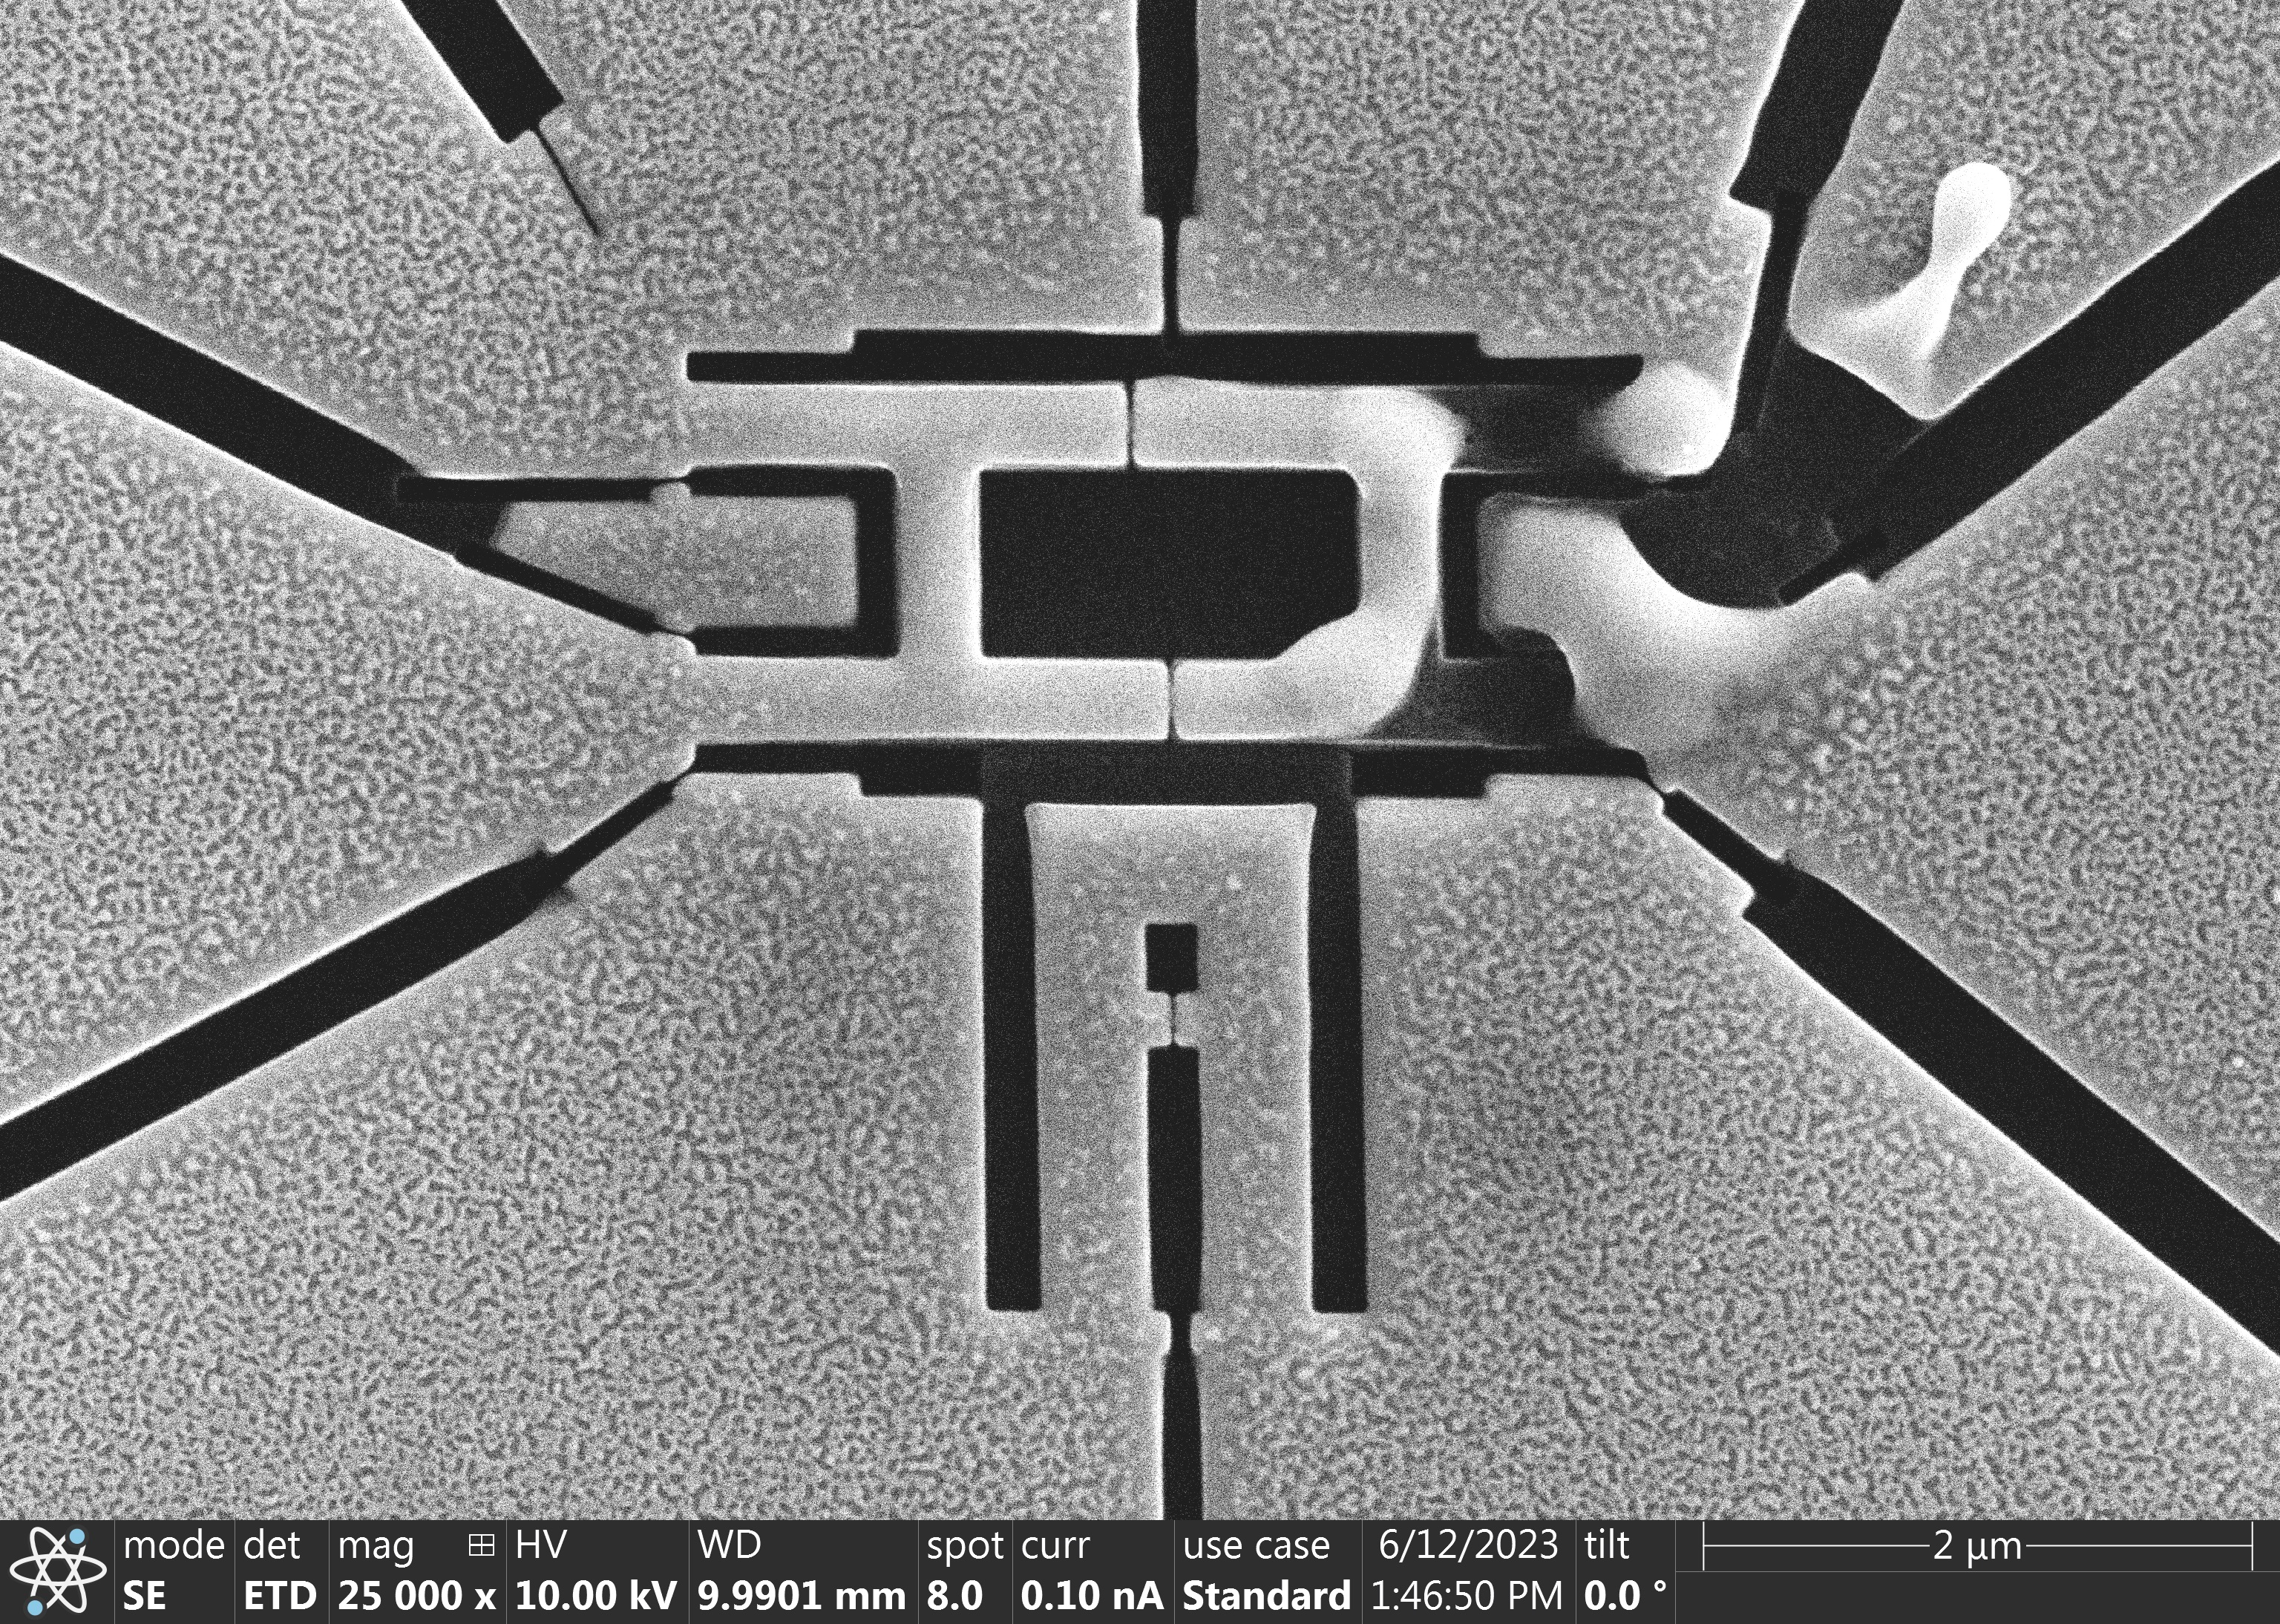
\includegraphics[width=0.5\textwidth]{figures/samples/CP3/CP3.5A_SEM_blown_up.jpg}
	\caption{The remains of sample CP3. Figure~\ref{fig:CP3.5A-SEM-images} shows what the sample originally looked like.}
	\label{fig:CP3.5A-remains}
\end{figure}

There is one noteworthy result for this sample. During our measurements it appeared as though the sample has two critical temperatures. The RT-curves are shown in Figure~\ref{fig:CP3.5A_RT_curves}. The bulk transition of the dc-SQUID appears to be around \qty{7.5}{\kelvin}. The junction's loop transitions around \qty{6}{\kelvin}. The results is particularly puzzling because the bulk sizes are the same; the materials were deposited simultaneously; and there were no significant exposure differences during FIB. Compared to the RT-curves of our previous sample it seems that the dc-SQUID is the outlier. Its resistance before the transition is much higher (almost \qty{20}{\ohm} compared to \qty{5}{\ohm}) and the critical temperature is higher than before. In hindsight we think the cause is a significant delay between the sample's thermometer and the sample itself. The delay has not been noted before as we took period measurements instead of waiting for temperature stability. This could easily be checked if it the sample was still alive.

\begin{figure}[ht!]
	\centering
	\input{figures/samples/CP3/CP3.5A_critical_temperature.pgf}
	\caption{Temperature dependences of the 4-point resistance measured over the dc-SQUID and the junction's loop. The inset shows the RT-curves from \qtyrange{0}{300}{\kelvin}. The main figure highlights the superconducting transitions. The junction's loop resistance is quite sharp. The dc-SQUID transition again has a `tail'. A reason for the difference in critical temperature is given in the main text.}
	\label{fig:CP3.5A_RT_curves}
\end{figure}

Regardless of these setbacks we do still think that the ideas behind the sample are promising. We suspect that the damage is caused by using two current sources in parallel. Future experiments might want to use a summing amplifier combined with a VI-converter or a Howland circuit.

\section{Sample CP2.6B revisited}
% !TEX root = ../../../thesis.tex
After the failure of sample CP3 we revisited sample CP2. By increasing the temperature it is possible to lower $I_c$. This opens the possibility to go into a non-hysteric regime by decreasing the screening parameter. Refer to Section~\ref{sec:CP3.5A-fabrication} for more information. The reason this was not attempted earlier is because the magnet controller was broken. As such it was not possible to measure SQIs at higher temperatures and consequently to measure the CPR at higher temperatures. The sample has not been altered, as such the reader is referred to Section~\ref{sec:CP2.6B-fabrication} for the geometries.

\subsection{Results and discussion}
% !TEX root = ../../../thesis.tex
The sample had not been permanently stored in a desiccator. An important check was thus if the sample had degraded. The RT-curve of the dc-SQUID showed no significant changes. As such it is unlikely that the sample degraded significantly. It also confirmed that all the contacts are still good.

Previously the CPR was measured at \qty{3}{\kelvin}. An increase in temperature degrades the sensitivity of our dc-SQUID and the critical current of the junction loop. We note that our measurement was approximately \qty{200}{\micro\ampere} periodic. In order to seem multiple periods it is preferable to have a critical junction around \qty{400}{\micro\ampere}. This allows us to see around 4 to 5 periods. Through trial and error we found the highest usable temperature to be \qty{3.4}{\kelvin}.

Similarly to last time we then measured SQIs for several bias currents. A bias current of \qtyrange{300}{350}{\micro\ampere} was used. They are shown in Figure~\ref{fig:CP2.6B_revisited_SQIs}. Whilst the SQIs are far from perfect, they are usable. The curved background is due to the magnetic field dependence of the critical current of the bulk.Near zero field the periodicity as well as the horizontal offset is reproducible. The amplitude of the oscillations is stable as well. Since the junction loop will only create a small flux this should be sufficient. Around zero field we can approximate the oscillations as sinusoidal. After fitting it gives a sensitivity of \qtylist{491.37;189.73;326.49;410.49;419.73}{\micro\volt\per\fluxquantum} for \qtylist{2.8;3.0;3.2;3.4;3.6}{\kelvin} respectively. These are comparable to previous results. Please note that the first sensitivity is significantly higher due to a higher bias current.

\begin{figure}[ht!]
	\centering
	\input{figures/samples/CP2/CP2.6B_revisited_SQIs.pgf}
	\caption{SQIs at \qtyrange{2.8}{3.6}{\kelvin} of sample CP2.6B. We note that they appear to have a slightly curved background. We used a bias current of \qty{300}{\micro\ampere} except for \qty{2.8}{\kelvin} where \qty{350}{\micro\ampere} was used. Near zero field the patterns seem quite stable but further out become more noisy.}
	\label{fig:CP2.6B_revisited_SQIs}
\end{figure}

After the calibrations the current-phase relations were measured. They are shown in Figure~\ref{fig:CP2.6B_revisited_CPRs}. The amplitude of the oscillations appears to decrease as the temperature increases. Except for the measurement at \qty{3.6}{\kelvin} where it increases again. We suspect that this is due to a human error. A likely explanation is that a different bias current was used for the dc-SQUID compared to the bias current used for the calibration. The change in amplitude corresponds to a change in critical current. Ignoring the measurement at \qty{3.6}{\kelvin}, the critical current goes from \qtyrange{90}{45}{\micro\ampere} between \qtyrange{2.8}{3.4}{\kelvin}. Besides the change in critical current we also note that the asymmetry changes. Both these changes are in line with theoretical models \cite{likharevSuperconductingWeakLinks1979}.

\begin{figure}[ht!]
	\centering
	\input{figures/samples/CP2/CP2.6B_revisited_CPRs.pgf}
	\caption{Various current-phase relations measured on sample CP2.6B in a range of \qtyrange{2.8}{3.6}{\kelvin}. The CPRs have been visually offset by \qty{150}{\micro\ampere}. The dashed lines denote zero current.}
	\label{fig:CP2.6B_revisited_CPRs}
\end{figure}

Previously we thought the steep curve was caused by a multivalued measurements. However, with these new results we think we wrong mainly because we see such a gradual transition.

Clearly the results show a few artefacts most notably at \qtylist{2.8;3.0;3.4}{\kelvin}. We attribute this to the fact that we are not in the linear regime of our dc-SQUID. We are confident that if the dc-SQUID would be biased in the linear regime that these artefacts would disappear. Additionally because we did not control our dc-SQUID's bias, it is not possible to say what point $\gamma = 0$. As such we have artificially centred the curves such that $\gamma = 0$ for $I_s=0$.

	% !TEX root = ../../thesis.tex
\chapter{Conclusion}
In this thesis a method to measure the current-phase relation of a Josephson junction was developed and its performance demonstrated. Our method utilises a dc-SQUID inductively coupled to a superconducting loop with a single junction. By passing a current through the junction's loop it is possible to modulate the phase of the junction. This phase is proportional to the flux in the loop which is measured by the dc-SQUID. From the total current and the measured flux the current-phase relation can be extracted.

The temperature dependence of the current-phase relation of a SNS junction was qualitatively determined using the above method. Starting from \qtyrange{2.8}{3.6}{\kelvin} the $2\pi$-periodic current-phase relation becomes more sinusoidal as the critical temperature is approached. Furthermore between \qtyrange{2.8}{3.4}{\kelvin} we determined the critical current to decrease from \qtyrange{90}{45}{\micro\ampere}. Both these observations are in line with theoretical models. However, the data does not yet allow us to distinguish between diffusive and ballistic behaviour.

Whilst successful, further improvements are possible. Most notably the implementation of a flux-locked loop. This will allow biasing the dc-SQUID at its working point. This means that the measurements will become more sensitive. Furthermore, a flux-locked loop allows integrating the results over a longer period improving the accuracy. An attempt was made to implement the flux-locked loop using a current modulation line. However, that sample was unfortunately destroyed. Future projects can use its design.

\section{Outlook}
The potential of the method has been demonstrated. Future research should improve the method. The most promising improvement is the addition of a flux-locked loop dc-SQUID readout scheme that improves the sensitivity and decreases unwanted background interference.  In order to measure the current-phase relation of \ce{Sr2RuO4} minor adjustments to the method are needed. It is impractical to make both the junction's loop and the dc-SQUID from the same crystal. But we can use our electron-beam-induced deposition facilities to directly deposit superconducting \ce{WC} next to the junction under study. Furthermore, we currently lack the knowledge on how to pin a single chiral domain wall. As such it is difficult to study a single chiral domain wall. Alternatively, it might be possible to incorporate a ring of \ce{Sr2RuO4} with two chiral domain walls instead of a single junction. In that case no additional weak links must be formed, or their behaviour negligible compared to the \ce{Sr2RuO4} ring.

	\appendix
	\chapter{Derivations}
	% !TEX root = ../../thesis.tex
\section{Phase-flux relation}
\label{app:phase-flux-relation}
We can write the magnetic field $\vec{B}$ as the curl of the magnetic vector potential $\vec{A}$. This allows us to rewrite the magnetic flux through the superconducting loop containing our junction in terms $\vec{A}$.
\begin{align}
	\Phi = \oiint \vec{B} \cdot d\vec{a} = \oiint \left(\nabla \times \vec{A}\right) \cdot d\vec{a} = \oint \vec{A} \cdot d\vec{l}
\end{align}
The closed integral over $\vec{A}$ can be any path enclosing the hole in the superconductor. It consists of two pieces, namely the junction and the rest of the loop.
\begin{align}
	\Phi = \int_{\text{JJ}} \vec{A} \cdot d\vec{l} + \int_{\text{loop}} \vec{A} \cdot d\vec{l}
	\label{eqn:magnetic-potential-integral}
\end{align}
For the integral over the junction we will use make use of the gauge-invariant phase (see Eq. \ref{eqn:gauge-invariant-phase}).
\begin{align}
	\gamma = \Delta\phi_{\text{JJ}} - \frac{2\pi}{\Phi_0}\int_{\text{JJ}}\vec{A} \cdot d\vec{l} \Rightarrow \int_{\text{JJ}}\vec{A} \cdot d\vec{l} = \frac{\Phi_0}{2\pi} \left(\Delta\phi_{\text{JJ}} - \gamma\right)
\end{align}
For the integral over the rest of the loop we will make use of the superfluid velocity\footnote{See \citetitle{tinkhamIntroductionSuperconductivity} equation 4.9, the equation has been converted to SI units.}:
\begin{equation}
	m^*\vec{v} = 2m_e\vec{v} = \hbar \nabla \varphi - \frac{e^*\vec{A}}{c} \stackrel{\text{SI}}{=} \hbar \nabla \varphi + 2e\vec{A}
	\label{eqn:superfluid-velocity}
\end{equation}
It allows us to rewrite:
\begin{align}
	\vec{A} = \frac{1}{2e}\left(\hbar \nabla \phi_{\text{loop}} - 2m_e\vec{v}\right)
\end{align}
We can substitute $\vec{v}$ with a more useable expression in terms of the current density $\vec{J}$ and $\lambda$ using Eq. \ref{eqn:london-penetration-depth}.
\begin{align}
	\vec{J} = -2e|\psi|^2\vec{v} = -\frac{m_e}{\lambda^2e\mu_0}\vec{v} \Rightarrow \vec{v} = -\frac{\lambda^2e\mu_0}{m_e}\vec{J}
\end{align}
Combining the two equations gives us a useable expression for $\vec{A}$ in the loop:
\begin{align}
	\vec{A} &= \frac{1}{2e}\left(\hbar \nabla \phi_{\text{loop}} + 2\lambda^2e\mu_0\vec{J} \right) \nonumber \\
	&= \frac{\Phi_0}{2\pi} \nabla \phi_{\text{loop}} + \lambda^2\mu_0\vec{J}
\end{align}
We can now go back to Eq. \ref{eqn:magnetic-potential-integral}:
\begin{align}
	\Phi &= \underbrace{\frac{\Phi_0}{2\pi} \left(\gamma - \Delta\phi_{\text{JJ}}\right)}_{\int_{\text{JJ}}\vec{A} \cdot d\vec{l}} \underbrace{- \frac{\Phi_0}{2\pi}\Delta \phi_{\text{loop}} - \lambda^2\mu_0 \int \vec{J}\cdot d \vec{l}}_{\int_{\text{loop}}\vec{A}\cdot d\vec{l}} \nonumber \\
	&= \frac{\Phi_0}{2\pi} \left(\gamma - \underbrace{\left(\Delta\phi_{\text{JJ}} + \Delta\phi_{\text{loop}}\right)}_{\text{Multiple of } 2\pi} \right) - \lambda^2\mu_0 \int \vec{J}\cdot d \vec{l}
\end{align}
The phase must wind by a multiple of $2\pi$ to make sure that the wave function is uniquely defined at each point. Using this fact and the quantization of $\Phi$ in units of $\Phi_0$ we find:
\begin{align}
	\Phi &= \left(\frac{\Phi_0}{2\pi}\gamma - \lambda^2\mu_0 \int \vec{J}\cdot d \vec{l} \right) \mod \Phi_0 \\ 
	% \Rightarrow \gamma &= -\left(\frac{2\pi\Phi}{\Phi_0} + \frac{2\pi\lambda^2\mu_0}{\Phi_0} \int \vec{J}\cdot d \vec{l} \right) \mod 2\pi \\
	\gamma &= \frac{2\pi}{\Phi_0}\left(\Phi + \lambda^2\mu_0 \int \vec{J}\cdot d \vec{l} \right)
	\label{eqn:phase-flux-relation}
\end{align}
%	\chapter{Data}
%	% !TEX root = ../../thesis.tex
\section{CP2 data}
\label{app:CP2.6B-data}

	\printbibliography
\end{document}
